\chapter{Resultados} \label{chap:results}

%%%%%%%%%%%%%%%%%%%%%%%%%%%%%%%%%%%%%%%%%%%%%%%%%%%%%%%%%%%%%%%%%
% Índice 
%%%%%%%%%%%%%%%%%%%%%%%%%%%%%%%%%%%%%%%%%%%%%%%%%%%%%%%%%%%%%%%%% Resultados para cada uno de los objetivos específicos 

En este capítulo se exponen los resultados obtenidos con la metodología propuesta. La sección \ref{res:matriz} está dedicada a la matriz de tiempos de residencia. Esta se estimó en dos etapas; en primer lugar, usando la Encuesta Origen-Destino tratada mediante el algoritmo \ref{alg:timematrix} para obtener el comportamiento de los santiaguinos en condiciones normales. A continuación, se utilizan datos de movilidad para actualizar esta matriz, de forma que refleje las variaciones en pandemia.

En la sección \ref{sec:estimacion-results} se muestra la estimación del factor sanitario. Esto se hace en dos etapas; en primer lugar se calcula para un caso sintético, donde la solución buscada está disponible. El conjunto de parámetros que permite una buena recuperación del factor sanitario se extrapola al caso real, donde se utilizan los casos confirmados obtenidos de Datos-COVID19 presentados en la subsección \ref{sec:datos-minsal}. Se estudia además la sensibilidad de las estimaciones ante distintos parámetros.

Finalmente, en la sección \ref{sec:evalmodel-casoshipot}, se usan los valores estimados en la sección anterior para simular varios casos hipotéticos; ¿cómo habría sido el desarrollo de la pandemia si todos se cuidaran de la misma forma pero además pudieran guardar una cuarentena más estricta? ¿y si no se hacía cuarentena pero todos respetaban las medidas sanitarias de una mejor manera?.  Se estudian dos escenarios dados por el parámetro \(\beta_{\text{exterior}}\).
%En segundo lugar, en la subsección \ref{subsec:rt}, se calcula el valor del \(\mathcal{R}_t\) para Santiago, y se compara con valor calculado con el método de Cori \cite{Cori2013} por el Centro de Modelamiento Matemático.



% Resultados de la matriz con tiempo constantes 
\section{Matriz de tiempos de residencia} \label{res:matriz}

En esta sección se muestran las matrices de tiempos de residencia estimadas para la ciudad de Santiago. La estimación se hizo en dos etapas; en primer lugar se calcula una matriz en condiciones normales, antes de la llegada del virus, lo que se presenta en la subsección \ref{res:matrix-normal}. Preliminarmente se calculó una matriz muy granular, la cual es presentada pues es de interés en si misma. La versión a utilizar, sin embarago, es mucho más simple.

En la segunda etapa de la estimación, se utilizan datos de movilidad para modificar la matriz de condiciones normales, a fin de que refleje el comportamiento de la población en pandemia. Esto se presenta en la subsección \ref{res:matrix-pandemia}.

\subsection{Santiago en condiciones normales}\label{res:matrix-normal}

Originalmente se deseaba trabajar con una mayor cantidad de clases y ambientes. La idea era utilizar una clasificación por sexo, edad e ingresos familiares, e incluir una lista bastante extensa de ambientes; prácticamente todos los propósitos incluidos en la Encuesta Origen-Destino. Es por esto que se calculó una matriz granular de tiempos de residencia en condiciones normales, mediante el algoritmo \ref{alg:timematrix}. Los resultados son presentados en \ref{res:matrix-normal-detallada}.

Esta matriz, sin embargo, es demasiado detallada. Como se discutió en \ref{subsec:eleccion-clases-ambientes}, no se cuenta con los datos necesarios para actualizarla sin hacer una gran cantidad de supuestos, por lo que solamente se utilizarán \(n = 5\) clases y \(m = 2\) ambientes, hogar y exterior. Los resultados se muestran en \ref{res:matrix-normal-simulaciones}.

% El código para esta sección esta en el github...
El código en Matlab para esta sección se encuentra disponible en el repositorio de GitHub \url{https://github.com/tabitaCatalan/lagrangian-time}, más específicamente en el directorio \texttt{src/time\_residence\_matrix/}.

\subsubsection*{Matriz detallada}\label{res:matrix-normal-detallada}
% \noindent \textbf{Matriz detallada}\\

% Elección de clases y ambientes, lista de ambientes disponibles en la EOD, cómo se eligieron las clases, etc. Esto debería estar docuementado en el repo. 
% \ref{alg:timematrix} 
Se aplica el algoritmo \ref{alg:timematrix} a la Encuesta Origen-Destino Santiago 2012, ya descrita en \ref{sec:eod}. Las clases son elegidas combinando los tres criterios de la tabla \ref{table:clases-full}; tres niveles de edad, sexo y tres niveles socioeconómicos dan lugar a 18 clases. El nivel socioeconómico es calculado en base a los datos de ingreso de cada persona provistos por la encuesta, agrupando a nivel de hogar y dividiendo por la cantidad de habitantes del hogar. Los ingresos de corte son elegidos de tal forma que cada tramo socioeconómico tiene unas \(20\,000\) personas.

\begin{table}[h!]
\centering
\begin{tabular}{||r|c||c||r|c||} 
 \hline
 \multicolumn{2}{||c||}{\textbf{Edad (años)}} & \textbf{Sexo}      & \multicolumn{2}{c||}{\begin{tabular}{@{}c@{}}\textbf{Nivel Socioeconómico} \\ \textbf{(ingreso per cápita)}\end{tabular}} \\
 \hline
 Joven & 0-24   & Hombre    & Bajo&\(\leq\) \$\(111\,666\)\\
 Adulto & 25-64 & Mujer     & Medio& \$ \(111\,667\) - \$ \(199\,999 \)\\
 Mayor & 65 o más &         & Alto&\(\geq\) \$ \(200\,000\)\\
 \hline
\end{tabular}
\caption{Criterios usados para obtener las clases de la matriz detallada a partir de la EOD2012 Santiago.}
\label{table:clases-full}
\end{table}


Los ambientes utilizados están basados en la lista de propósitos de viajes y los modos de transporte usados. Son los siguientes: \texttt{hogar}, \texttt{trabajo}, \texttt{estudios}, \texttt{compras}, \texttt{visitas}, \texttt{salud}, \texttt{trámites}, \texttt{recreación}, \texttt{transporte público}, \texttt{auto}, \texttt{caminata}, \texttt{bicicleta} y \texttt{otros}. La lista de propósitos de viajes y sus ambientes asociados se encuentra en la tabla \ref{table:ambientes-prop-full}. La lista de modos está en la tabla \ref{table:ambientes-modo-full}.

% \begin{table}[h!]
% \centering
% \begin{tabular}{||l|c||l|c||} 
%  \hline
%  \multicolumn{2}{||c||}{Propósito de viaje} &  \multicolumn{2}{c||}{Modo de transporte} \\
%  \hline
% 1. Al trabajo               & \texttt{trabajo}      & 1:Auto                        & \texttt{auto}\\
% 2. Por trabajo              & \texttt{trabajo}      & 2:Bus TS                      & \texttt{transporte público}\\
% 3. Al estudio               & \texttt{estudios}     & 3:Bus no TS                   & \texttt{transporte público}\\
% 4. Por estudio              & \texttt{estudios}     & 4:Metro                       & \texttt{transporte público}\\
% 5. De salud                 & \texttt{salud}        & 5:Taxi Colectivo              & \texttt{transporte público}\\
% 6. Visitar a alguien        & \texttt{visitas}      & 6:Taxi                        & \texttt{auto}\\
% 7. Volver a casa            & \texttt{hogar}        & 7:Bus TS - Bus no TS          & \texttt{transporte público}\\
% 8. Buscar o dejar a alguien & \texttt{visitas}      & 8:Auto - Metro                & \texttt{transporte público}\\
% 9. Comer o tomar algo       & \texttt{compras}      & 9:Bus TS - Metro              & \texttt{transporte público}\\
% 10.Buscar o dejar algo      & \texttt{compras}      & 10:Bus no TS - Metro          & \texttt{transporte público}\\
% 11.De compras               & \texttt{compras}      & 11:Taxi Colectivo - Metro     & \texttt{transporte público}\\
% 12.Tramites                 & \texttt{trámites}     & 12:Taxi - Metro               & \texttt{transporte público}\\
% 13.Recreación               & \texttt{recreación}   & 13:Otros - Metro              & \texttt{transporte público}\\
% 14.Otra actividad           & \texttt{otros}        & 14:Otros - Bus TS             & \texttt{transporte público}\\
%                             &                       & 15:Otros - Bus TS - Metro     & \texttt{transporte público}\\
%                             &                       & 16:Otros                      & \texttt{otros}\\
%                             &                       & 17:Caminata                   & \texttt{caminata}\\
%                             &                       & 18:Bicicleta                  & \texttt{bicicleta}\\
%  \hline
% \end{tabular}
% \caption{Propósitos de viaje y modos de transporte de la EOD2012, y sus ambientes asociados.}
% \label{table:ambientes-full}
% \end{table}

\begin{table}[h!]
\centering
\begin{tabular}{||l|c||} 
 \hline
 \multicolumn{2}{||c||}{\textbf{Propósito de viaje}} \\
 \hline
1. Al trabajo               & \texttt{trabajo}      \\
2. Por trabajo              & \texttt{trabajo}      \\
3. Al estudio               & \texttt{estudios}     \\
4. Por estudio              & \texttt{estudios}     \\
5. De salud                 & \texttt{salud}        \\
6. Visitar a alguien        & \texttt{visitas}      \\
7. Volver a casa            & \texttt{hogar}        \\
8. Buscar o dejar a alguien & \texttt{visitas}      \\
9. Comer o tomar algo       & \texttt{compras}      \\
10.Buscar o dejar algo      & \texttt{compras}      \\
11.De compras               & \texttt{compras}      \\
12.Tramites                 & \texttt{trámites}     \\
13.Recreación               & \texttt{recreación}   \\
14.Otra actividad           & \texttt{otros}        \\
 \hline
\end{tabular}
\caption[Propósitos de viaje de la EOD2012 y sus ambientes asociados.]{Propósitos de viaje de la EOD2012 y sus ambientes asociados, lo que permite definir \(\mathcal{J}_{\mathtt{p}}\).}
\label{table:ambientes-prop-full}
\end{table}

\begin{table}[h!]
\centering
\begin{tabular}{||l|c||} 
 \hline
 \multicolumn{2}{||c||}{\textbf{Modo de transporte}} \\
 \hline
 1:Auto                        & \texttt{auto}\\
 2:Bus TS                      & \texttt{transporte público}\\
 3:Bus no TS                   & \texttt{transporte público}\\
 4:Metro                       & \texttt{transporte público}\\
 5:Taxi Colectivo              & \texttt{transporte público}\\
 6:Taxi                        & \texttt{auto}\\
 7:Bus TS - Bus no TS          & \texttt{transporte público}\\
 8:Auto - Metro                & \texttt{transporte público}\\
 9:Bus TS - Metro              & \texttt{transporte público}\\
 10:Bus no TS - Metro          & \texttt{transporte público}\\
 11:Taxi Colectivo - Metro     & \texttt{transporte público}\\
 12:Taxi - Metro               & \texttt{transporte público}\\
 13:Otros - Metro              & \texttt{transporte público}\\
 14:Otros - Bus TS             & \texttt{transporte público}\\
 15:Otros - Bus TS - Metro     & \texttt{transporte público}\\
 16:Otros                      & \texttt{otros}\\
 17:Caminata                   & \texttt{caminata}\\
 18:Bicicleta                  & \texttt{bicicleta}\\
 \hline
\end{tabular}
\caption[Modos de transporte de la EOD2012 y sus ambientes asociados.]{Modos de transporte de la EOD2012 y sus ambientes asociados, lo que permite definir \(\mathcal{J}_{\mathtt{m}}\).}
\label{table:ambientes-modo-full}
\end{table}

La matriz obtenida se presenta en la figura \ref{img:Pmatrix-full}. Como era de esperarse, todas las clases pasan la mayor parte de su tiempo en el hogar, de hecho, se redujo el tiempo en el hogar en 7 horas, asociadas al de tiempo de sueño, y se volvió a normalizar la matriz por filas, de forma que las proporciones de tiempo por clase siguieran sumando 1.

De esta matriz pueden hacerse algunas observaciones. Los adultos pasan una cantidad considerable de tiempo en el trabajo, en especial los hombres. Los jóvenes pasan mucho tiempo en el ambiente estudios, especialmente los de clase alta; los jóvenes con menos ingresos pasan más tiempo en el trabajo. Los adultos mayores pasan mucho más tiempo en el hogar, pero los hombres pasan una cantidad importante de tiempo en el trabajo. 

El nivel socioeconómico medio pasa menos tiempo de compras y de visita que los demás. Los adultos mayores son quienes pasan más tiempo en el ambiente salud, especialmente los de clase baja. El auto es bastante más utilizado por la clase alta y por los adultos hombres de clase media, mientras que el transporte público es más predominante en adultos de la clase media y baja.

En general los resultados son los esperados para una ciudad con una segregación importante como lo es Santiago. Es posible que en la última década se haya reducido la brecha de género, pero eso queda fuera del alcance de este trabajo.


\begin{figure}[!h]
\centering
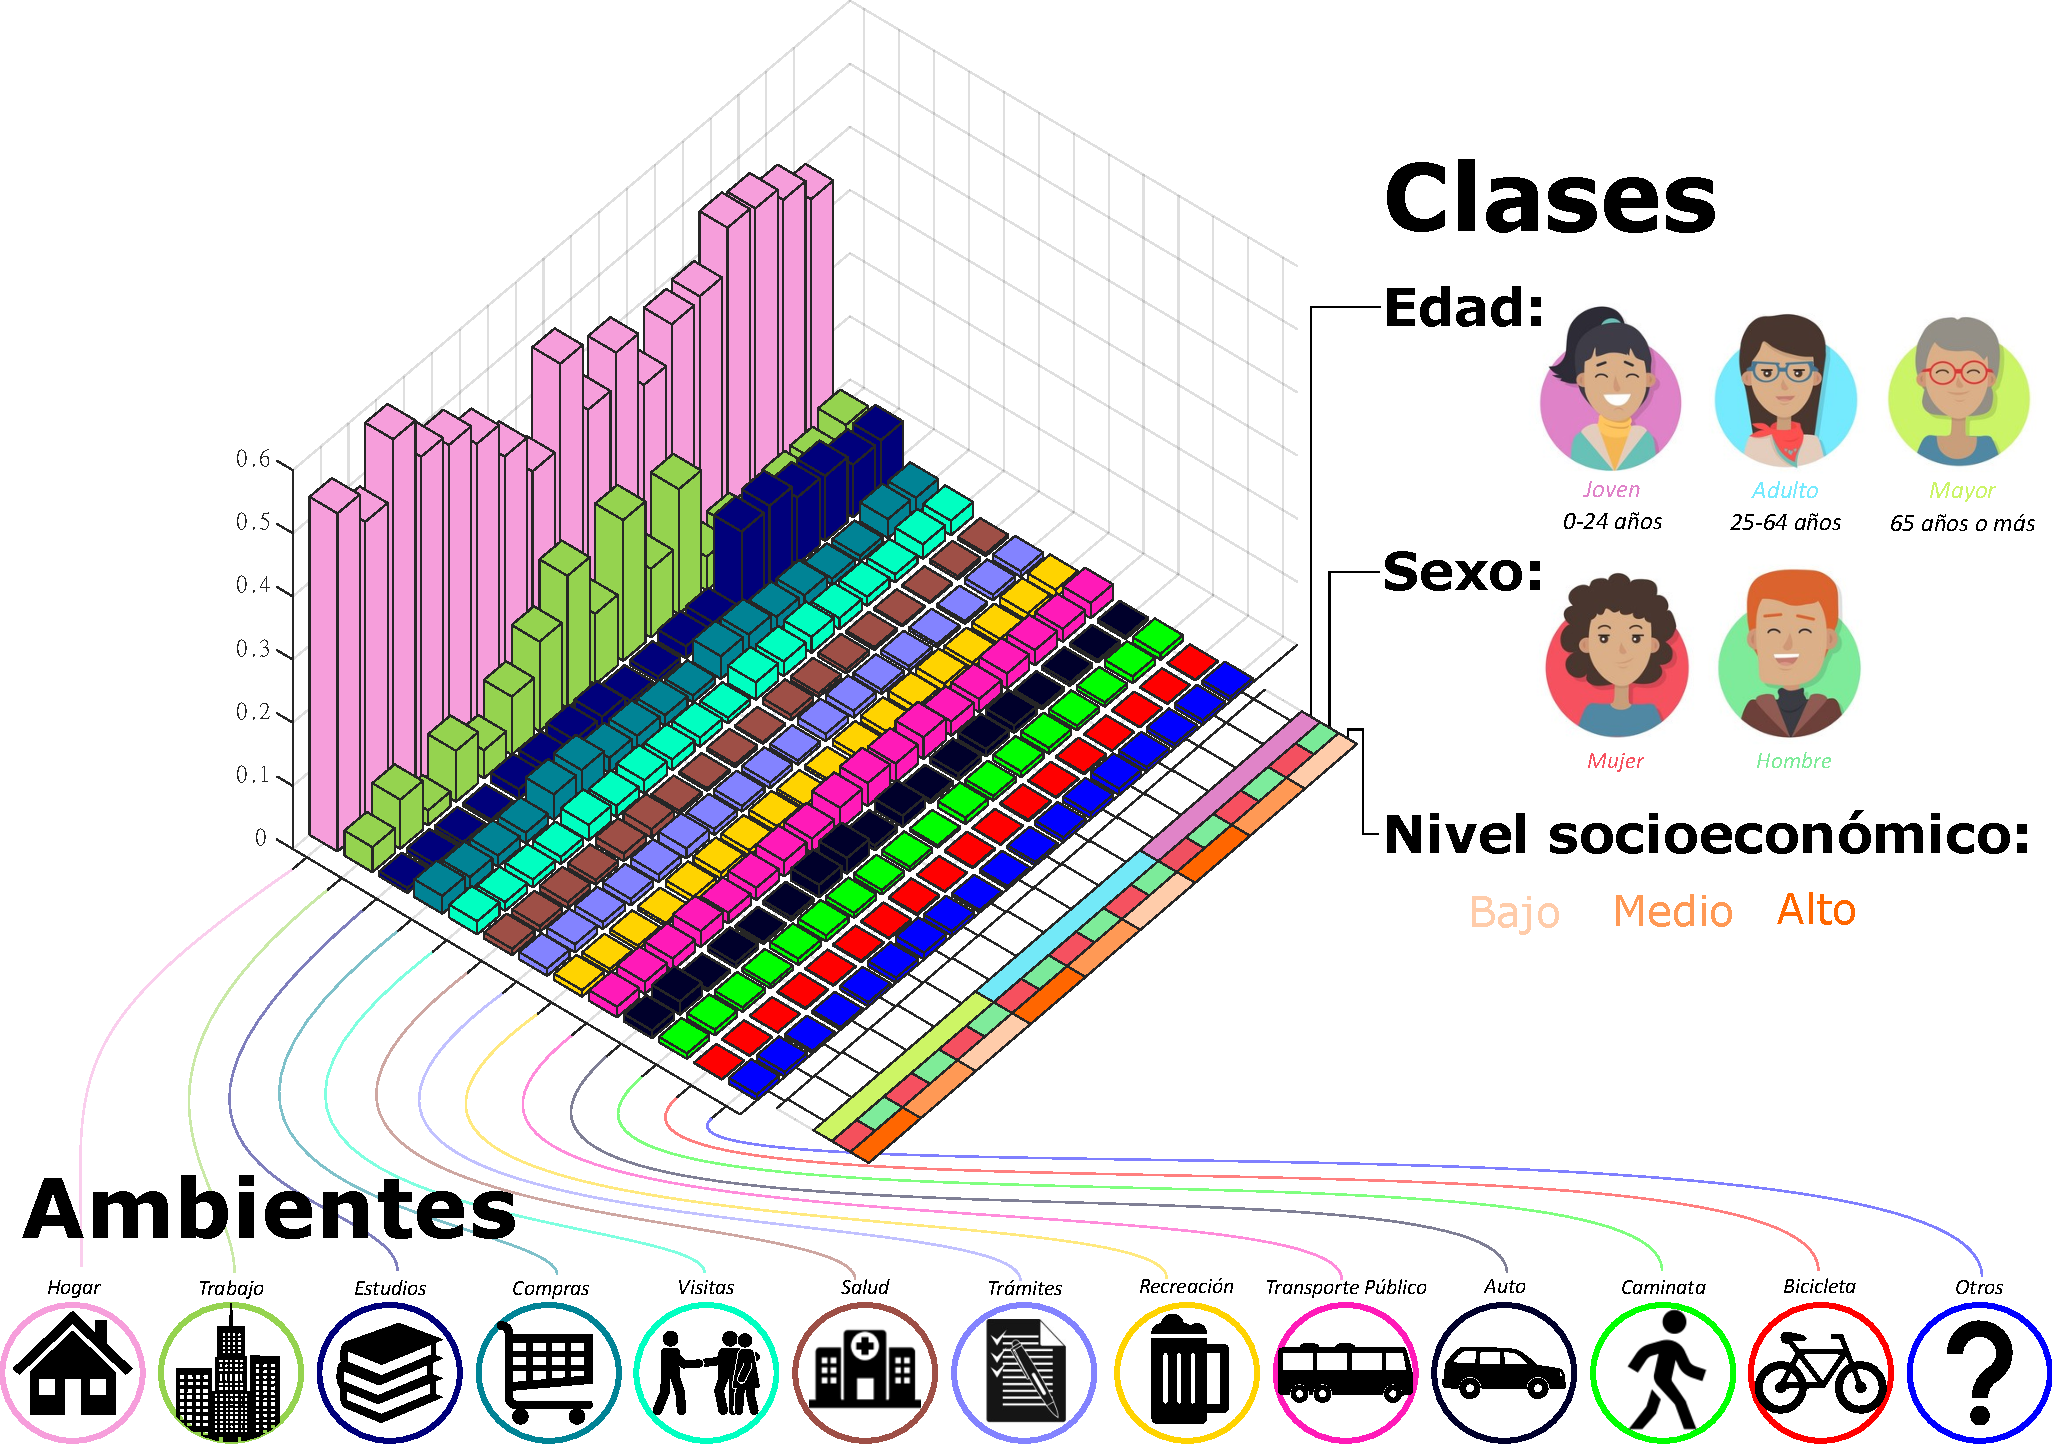
\includegraphics[width=0.99\textwidth]{img/resultados/matrixP/matriz Pambientesyclases.pdf}
\caption[Matriz detallada de tiempos de residencia para Santiago]{Matriz detallada de tiempos de residencia para Santiago. Considera clases basadas en nivel socioeconómico (según ingreso promedio del hogar), edad y sexo. 13 ambientes, basados en los propósitos de viajes de la encuesta. Se restan 7 horas del tiempo en el hogar (tiempo de sueño) y se normalizan las filas para que sumen 1.}
\label{img:Pmatrix-full}
\end{figure}

\subsubsection*{Matriz para las simulaciones}\label{res:matrix-normal-simulaciones}
%\noindent \textbf{Matriz para las simulaciones}

La aplicación del algoritmo tomando en consideración las decisiones tomadas en la sección \ref{subsec:eleccion-clases-ambientes}, específicamente la elección de 5 clases agrupadas por IPS como se detalla en la tabla \ref{table:ips-categ}, y del uso de los ambientes \texttt{hogar} y \texttt{exterior}. Se obtiene una matriz de tiempos de residencia \(P^0\) mucho más sencilla, presentada en la tabla \ref{table:matrix-simulaciones}.

\begin{table}[h!]
\centering
\begin{tabular}{||c c | c c ||} 
 \hline
 \textbf{Clase} & \textbf{Prioridad Social} &  \(P^0_{:,\text{hogar}}\) & \(P^0_{:,\text{exterior}}\)\\[1ex] 
 \hline
 1 & Sin Prioridad  & 0.73  & 0.27 \\ 
 2 & Baja           & 0.76  & 0.24 \\
 3 & Media Baja     & 0.77  & 0.23 \\
 4 & Media Alta     & 0.77  & 0.23 \\
 5 & Alta           & 0.77  & 0.23 \\ 
 \hline
\end{tabular}
\caption[Matriz de tiempos de residencia para las simulaciones.]{Matriz de tiempos de residencia para las simulaciones. La clase sin prioridad corresponde a la más acomodada y la clase con prioridad alta a la más vulnerable.}
\label{table:matrix-simulaciones}
\end{table}

\subsection{Santiago a lo largo del tiempo} \label{res:matrix-pandemia}

Una vez que una matriz \(P^0\) ha sido calculada, se requiere modificar esta matriz a fin de obtener \(P(t)\) que refleje el comportamiento de la población en pandemia. Estas modificaciones se hacen utilizando los datos de movilidad, siguiendo la metodología presentada en \ref{subsec:variaciones}; los datos de movilidad comunal son agregados ponderando por la población de la comuna, y suponiendo que la movilidad inicial era la misma en cada grupo.

La figura \ref{img:mov-pandemia} muestra la variación de movilidad para los distintos grupos socioeconómicos con respecto a la movilidad de la semana base. Se observa que la línea para la clase Sin Prioridad, es decir, la más acomodada, se mantiene por debajo de las otras, lo que significa que logró reducir su movilidad mucho más.

\begin{figure}[H]
\centering
\begin{subfigure}[b]{0.8\textwidth}
     \centering
     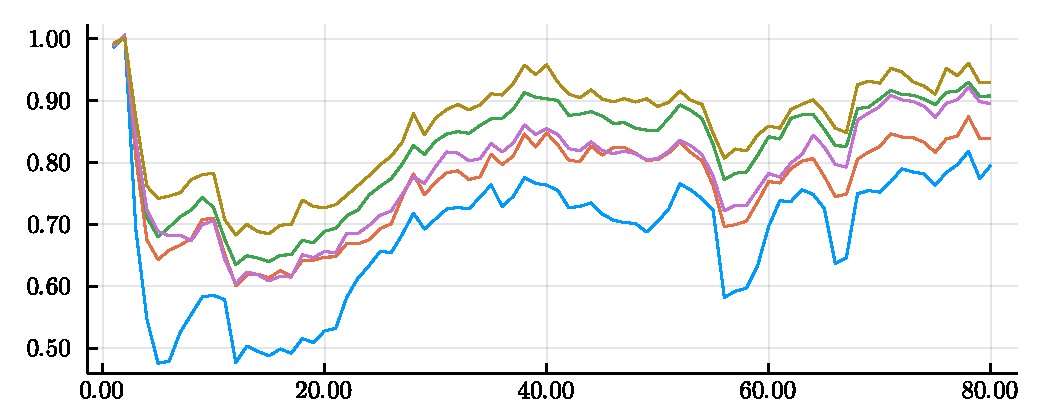
\includegraphics[width=0.99\textwidth]{img/resultados/mob-reduction.pdf}
\end{subfigure} 
\hfill
\begin{subfigure}[b]{0.99\textwidth}
 \centering
\scalebox{0.7}{
\begin{tikzpicture}
	\begin{pgfonlayer}{nodelayer}
		\node [style=none] (50) at (5, 0) {};
		\node [style=none] (51) at (7, 0) {};
		\node [style=none] (52) at (6, -0.5) {Prioridad Alta};
		\node [style=none] (53) at (2, 0) {};
		\node [style=none] (54) at (4, 0) {};
		\node [style=none] (55) at (3, -0.5) {Prioridad};
		\node [style=none] (56) at (-1, 0) {};
		\node [style=none] (57) at (1, 0) {};
		\node [style=none] (58) at (0, -0.5) {Prioridad};
		\node [style=none] (59) at (-4, 0) {};
		\node [style=none] (60) at (-2, 0) {};
		\node [style=none] (61) at (-3, -0.5) {Prioridad Baja};
		\node [style=none] (62) at (-7, 0) {};
		\node [style=none] (63) at (-5, 0) {};
		\node [style=none] (64) at (-6, -0.5) {Sin Prioridad};
		\node [style=none] (65) at (0, -1) {Media Baja};
		\node [style=none] (66) at (3, -1) {Media Alta};
	\end{pgfonlayer}
	\begin{pgfonlayer}{edgelayer}
		\draw [style=class5] (50.center) to (51.center);
		\draw [style=class1] (62.center) to (63.center);
		\draw [style=class2] (59.center) to (60.center);
		\draw [style=class3] (56.center) to (57.center);
		\draw [style=class4] (53.center) to (54.center);
	\end{pgfonlayer}
\end{tikzpicture}

}
\end{subfigure}
\caption[Fracción de la movilidad en pandemia por clase, c/r a movilidad normal.]{Fracción de la movilidad en pandemia por grupos, con respecto a la movilidad normal. Se considera la semana base como la correspondiente a 02/mar/2020 - 06/mar/2020.}
\label{img:mov-pandemia}
\end{figure}

 Ahora bien, al combinar esos datos con los de \ref{res:matrix-normal-simulaciones} se obtiene la imagen \ref{img:Pmatrix-pandemia-exterior}, que representa el tiempo de residencia estimado en el ambiente \texttt{exterior}. Se puede ver que, para la clases más acomodada, el mayor tiempo que pasan en el exterior compensa su mayor reducción de movilidad, haciendo menos notarias las diferencias.


\begin{figure}[!h]
\centering
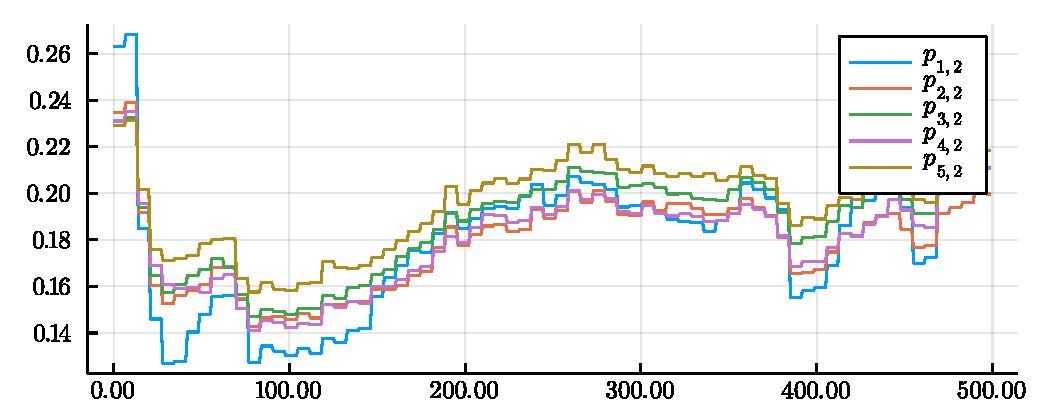
\includegraphics[width=0.8\textwidth]{img/resultados/tiempos-exterior.pdf}
\caption[Tiempo de residencia en \texttt{exterior} para las 5 clases elegidas.]{Tiempo de residencia en \texttt{exterior} para las 5 clases elegidas, desde 02/mar/2020.}
\label{img:Pmatrix-pandemia-exterior}
\end{figure}



\section{Análisis de sensibilidad}


\begin{figure}
\centering
\begin{tikzpicture}
	\begin{pgfonlayer}{nodelayer}
		\node [style=none] (0) at (-2, 2) {};
		\node [style=none] (1) at (0, 2) {};
		\node [style=none] (2) at (-2, 1) {};
		\node [style=none] (3) at (0, 1) {};
		\node [style=none] (4) at (-2, 0) {};
		\node [style=none] (5) at (0, 0) {};
		\node [style=none] (6) at (-2, -1) {};
		\node [style=none] (7) at (0, -1) {};
		\node [style=none] (8) at (2, 2) {$0.15$};
		\node [style=none] (9) at (2, 1) {};
		\node [style=none] (10) at (2, 1) {};
		\node [style=none] (11) at (2, 1) {$0.25$};
		\node [style=none] (12) at (2, 0) {};
		\node [style=none] (13) at (2, 0) {$0.35$};
		\node [style=none] (14) at (2, -1) {};
		\node [style=none] (15) at (2, -1) {$0.45$};
		\node [style=none] (16) at (0, 3) {};
		\node [style=none] (17) at (0, 3) {Condición inicial $\alpha_0$};
		\node [style=none] (18) at (6, 3) {};
		\node [style=none] (19) at (6, 3) {$\beta_{\textrm{ext}}$};
		\node [style=none] (20) at (0, -3) {};
		\node [style=none] (21) at (0, -3) {Solución real};
		\node [style=none] (22) at (-2, -4) {};
		\node [style=none] (23) at (0, -4) {};
		\node [style=none] (24) at (2, -4) {};
		\node [style=none] (25) at (2, -4) {$1.88$};
		\node [style=none] (26) at (4, 2) {};
		\node [style=none] (27) at (6, 2) {};
		\node [style=none] (28) at (4, 1) {};
		\node [style=none] (29) at (6, 1) {};
		\node [style=none] (30) at (4, 0) {};
		\node [style=none] (31) at (6, 0) {};
		\node [style=none] (32) at (4, -1) {};
		\node [style=none] (33) at (6, -1) {};
		\node [style=none] (34) at (4, -2) {};
		\node [style=none] (35) at (6, -2) {};
		\node [style=none] (36) at (4, -3) {};
		\node [style=none] (37) at (6, -3) {};
		\node [style=none] (38) at (4, -4) {};
		\node [style=none] (39) at (6, -4) {};
		\node [style=none] (40) at (4, -5) {};
		\node [style=none] (41) at (6, -5) {};
		\node [style=none] (42) at (8, 2) {$1.2$};
		\node [style=none] (43) at (8, 1) {$1.5$};
		\node [style=none] (44) at (8, 0) {$1.8$};
		\node [style=none] (45) at (8, -1) {$2.1$};
		\node [style=none] (46) at (8, -2) {$2.4$};
		\node [style=none] (47) at (8, -3) {$2.7$};
		\node [style=none] (48) at (8, -4) {$3.0$};
		\node [style=none] (49) at (8, -5) {$3.3$};
	\end{pgfonlayer}
	\begin{pgfonlayer}{edgelayer}
		\draw [style={a0_1}] (0.center) to (1.center);
		\draw [style={a0_2}] (2.center) to (3.center);
		\draw [style={a0_3}] (4.center) to (5.center);
		\draw [style={a0_4}] (6.center) to (7.center);
		\draw [style=real] (22.center) to (23.center);
		\draw [style=beta1] (26.center) to (27.center);
		\draw [style=beta2] (28.center) to (29.center);
		\draw [style=beta3] (30.center) to (31.center);
		\draw [style=beta4] (32.center) to (33.center);
		\draw [style=beta5] (34.center) to (35.center);
		\draw [style=beta6] (36.center) to (37.center);
		\draw [style=beta7] (38.center) to (39.center);
		\draw [style=beta8] (40.center) to (41.center);
	\end{pgfonlayer}
\end{tikzpicture}

\caption{Leyenda sensibilidad ante \(\beta_{\text{exterior}}\).} \label{fig:legend-sensi-b}
\end{figure}



% Resultados de usar el filtro de kalman 
\section{Estimación de parámetros}\label{sec:estimacion-results}

En todos los resultados presentados se utiliza \(\Delta t = 1 \text{día}\). Se probó con valores más pequeños sin alterar el desempeño del método.

%\subsection{Modelo con una clase}
\subsection{Modelo multiclase con datos sintéticos} \label{subsec:sintetico}

Se utilizan los datos de movilidad de dos comunas (San Bernardo y las Condes) para generar las matrices de tiempos de residencia variables en el tiempo. Se fijan valores \(\gamma_E = 1/5.1, \gamma_I = 1/8.2\) y condiciones iniciales... Se fija riesgos \(\beta_{\text{hogar}} = 1\) y \(\beta_{\text{exterior}} = 1.88\). 

Mediante prueba y error se genera dos controles diferentes para cada clase, de forma que el total de casos acumulados tengan órdenes de magnitud similares a los datos reales.

A partir de la solución de la ecuación diferencial es posible obtener las series \(C_1, C_2\). Las observaciones son obtenidas con \(\Delta t = 1\) [día]. Se utilizan estas observaciones directamente (sin añadir ruido), y el filtro asume que tienen un ruido pequeño (G = diag(10)...). 

Se suponen condiciones iniciales diferentes a las utilizadas en la solución (...), y se eligen matrices de covarianza de tal forma de obtener resultados razonables. Un ejemplo de las estimaciones de estado obtenidas puede verse en la figura \ref{synth-all-nohigh}.



\begin{figure}[!h]
\centering
\includegraphics[width=0.99\textwidth]{img/resultados/synth/kalman_grouped_allstates_allgroups\parameterstring}
\caption{Ejemplo de estimación de estados y parámetros variables en el tiempo con \textit{Kalman Smoother}, a partir de las observaciones del número de casos acumulados \(C_1, C_2\).}
\label{synth-all-nohigh}
\end{figure}

Las matrices de covarianza iniciales son elegidas de modo tal que las soluciones reales quedan a una desviación estándar de la estimación, como se ve en la figura \ref{synth-e-comp-high}.


\begin{figure}[!h]
     \centering
     \begin{subfigure}[b]{\textwidth}
         \centering
         \includegraphics[width=.8\textwidth]{img/resultados/synth/kalman_grouped_E_high1\parameterstring}
         \caption{Clase \(1\).}
     \end{subfigure}
     \hfill
     \begin{subfigure}[b]{\textwidth}
         \centering
         \includegraphics[width=0.8\textwidth]{img/resultados/synth/kalman_grouped_E_high2\parameterstring}
         \caption{Clase \(2\).}
     \end{subfigure}
        \caption{Casos Expuestos, comparando resultados obtenidos con solución real, en valores absolutos y normalizados con respecto a la cantidad de personas por clase.}
        \label{synth-e-comp-high}
\end{figure}


Como se ve en la figura \ref{synth-alpha-comp-high}, es posible estimar el factor sanitario a partir de los datos, con ciertas consideraciones. En las secciones siguientes  se hablará en más detalle de la sensibilidad de la estimación con respecto a los parámetros del filtro. Más específicamente, se estudia la sensibilidad de la estimación del factor sanitario con respecto al parámetro \(\beta_{\text{exterior}}\) y la condición inicial. Se recuerda que se hizo la simplificación de que los ruidos en la dinámica son independientes, es decir que el ruido está dado por una matriz normal multivariada con matriz de covarianzas diagonal. Nos interesa por tanto, solo la diagonal de la matriz, las varianzas. Se muestra el efecto en la estimación al usar distintos valores para la matriz de varianzas.

\begin{figure}[!h]
     \centering
     \begin{subfigure}[b]{\textwidth}
         \centering
         \includegraphics[width=.99\textwidth]{img/resultados/synth/kalman_grouped_alpha_high1\parameterstring}
         \caption{Clase \(1\).}
     \end{subfigure}
     \hfill
     \begin{subfigure}[b]{\textwidth}
         \centering
         \includegraphics[width=0.99\textwidth]{img/resultados/synth/kalman_grouped_alpha_high2\parameterstring}
         \caption{Clase \(2\).}
     \end{subfigure}
        \caption[Factor sanitario, caso sintético]{Factor sanitario, comparando resultados obtenidos con función de control usada para general los datos, acotando el dominio en el eje \(y\) para mejor apreciación.}
        \label{synth-alpha-comp-high}
\end{figure}


\subsection{Sensibilidad con respecto a \(\beta_{\text{exterior}}\) y \(\alpha_0\)} \label{subsec:sensibeta}

\begin{figure}[H]
\centering
\begin{subfigure}[b]{0.47\textwidth}
     \centering
     \includegraphics[width=\textwidth]{img/resultados/synth/\stringsensiparam_high1_\stringrealandcovsparam\stringparamtwo.pdf}
     \caption{Estimación control clase 1, suponiendo conocidos \(\gamma_E = 1/5.1\) y \(\gamma_I = 1/7.2\)}
     \label{fig:legend-sensi-b-class1-gamma_real}
\end{subfigure} 
\hfill
\begin{subfigure}[b]{0.47\textwidth}
     \centering
     \includegraphics[width=\textwidth]{img/resultados/synth/\stringsensiparam_high2_\stringrealandcovsparam\stringparamtwo.pdf}
     \caption{Estimación control clase 2,  suponiendo conocidos \(\gamma_E = 1/5.1\) y \(\gamma_I = 1/7.2\)}
     \label{fig:legend-sensi-b-class2-gamma_real}
\end{subfigure} 
\hfill
\begin{subfigure}[b]{0.47\textwidth}
     \centering
     \includegraphics[width=\textwidth]{img/resultados/synth/\stringsensiparam_high1_\stringrealandcovsparam\stringparamthree.pdf}
     \caption{Estimación control clase 1,  con \(\gamma_E = 1/5.8\) y \(\gamma_I = 1/8.2\)}
     \label{fig:legend-sensi-b-class1-gamma_estimado}
\end{subfigure} 
\hfill
\begin{subfigure}[b]{0.47\textwidth}
     \centering
     \includegraphics[width=\textwidth]{img/resultados/synth/\stringsensiparam_high2_\stringrealandcovsparam\stringparamthree.pdf}
     \caption{Estimación control clase 2,  con \(\gamma_E = 1/5.8\) y \(\gamma_I = 1/8.2\)}
     \label{fig:legend-sensi-b-class2-gamma_estimado}
\end{subfigure} 
\hfill
\begin{subfigure}[b]{0.75\textwidth}
 \centering
\scalebox{0.7}{
\begin{tikzpicture}
	\begin{pgfonlayer}{nodelayer}
		\node [style=none] (0) at (-0.5, 1.25) {};
		\node [style=none] (1) at (1, 1.25) {};
		\node [style=none] (2) at (-0.5, 0.75) {};
		\node [style=none] (3) at (1, 0.75) {};
		\node [style=none] (4) at (-0.5, 0.25) {};
		\node [style=none] (5) at (1, 0.25) {};
		\node [style=none] (6) at (-0.5, -0.25) {};
		\node [style=none] (7) at (1, -0.25) {};
		\node [style=none] (8) at (1.5, 1.25) {$0.15$};
		\node [style=none] (9) at (1.5, 0.75) {};
		\node [style=none] (10) at (1.5, 0.75) {};
		\node [style=none] (11) at (1.5, 0.75) {$0.25$};
		\node [style=none] (12) at (1.5, 0.25) {};
		\node [style=none] (13) at (1.5, 0.25) {$0.35$};
		\node [style=none] (15) at (1.5, -0.25) {$0.45$};
		\node [style=none] (17) at (0.5, 1.75) {Condición inicial $\alpha_0$};
		\node [style=none] (19) at (12.5, 2.5) {$\beta_{\textrm{ext}}$};
		\node [style=none] (21) at (6.5, 1) {$\beta_{\text{ext}}$ solución real};
		\node [style=none] (22) at (5.5, 0.5) {};
		\node [style=none] (23) at (7, 0.5) {};
		\node [style=none] (24) at (7.5, 0.5) {};
		\node [style=none] (25) at (7.5, 0.5) {$1.88$};
		\node [style=none] (26) at (11.5, 2) {};
		\node [style=none] (27) at (13, 2) {};
		\node [style=none] (28) at (11.5, 1.5) {};
		\node [style=none] (29) at (13, 1.5) {};
		\node [style=none] (30) at (11.5, 1) {};
		\node [style=none] (31) at (13, 1) {};
		\node [style=none] (32) at (11.5, 0.5) {};
		\node [style=none] (33) at (13, 0.5) {};
		\node [style=none] (34) at (11.5, 0) {};
		\node [style=none] (35) at (13, 0) {};
		\node [style=none] (36) at (11.5, -0.5) {};
		\node [style=none] (37) at (13, -0.5) {};
		\node [style=none] (38) at (11.5, -1) {};
		\node [style=none] (39) at (13, -1) {};
		\node [style=none] (40) at (11.5, -1.5) {};
		\node [style=none] (41) at (13, -1.5) {};
		\node [style=none] (42) at (13.5, 2) {$1.2$};
		\node [style=none] (43) at (13.5, 1.5) {$1.5$};
		\node [style=none] (44) at (13.5, 1) {$1.8$};
		\node [style=none] (45) at (13.5, 0.5) {$2.1$};
		\node [style=none] (46) at (13.5, 0) {$2.4$};
		\node [style=none] (47) at (13.5, -0.5) {$2.7$};
		\node [style=none] (48) at (13.5, -1) {$3.0$};
		\node [style=none] (49) at (13.5, -1.5) {$3.3$};
	\end{pgfonlayer}
	\begin{pgfonlayer}{edgelayer}
		\draw [style={a0_1}] (0.center) to (1.center);
		\draw [style={a0_2}] (2.center) to (3.center);
		\draw [style={a0_3}] (4.center) to (5.center);
		\draw [style={a0_4}] (6.center) to (7.center);
		\draw [style=real] (22.center) to (23.center);
		\draw [style=beta1] (26.center) to (27.center);
		\draw [style=beta2] (28.center) to (29.center);
		\draw [style=beta3] (30.center) to (31.center);
		\draw [style=beta4] (32.center) to (33.center);
		\draw [style=beta5] (34.center) to (35.center);
		\draw [style=beta6] (36.center) to (37.center);
		\draw [style=beta7] (38.center) to (39.center);
		\draw [style=beta8] (40.center) to (41.center);
	\end{pgfonlayer}
\end{tikzpicture}
}
\end{subfigure}

\caption[Sensibilidad ante riesgo exterior y condición inicial del factor sanitario.]{Sensibilidad ante riesgo exterior y condición inicial del factor sanitario. Cada color representa un condición inicial diferente usada en la estimación, mientras que la opacidad de la solución representa la distancia de \(\beta_{\text{exterior}}\) al valor real; a mayor transparencia, más lejano.} \label{fig:legend-sensi-b}
\end{figure}

Los riesgos \(\beta \), las tasas \(\gamma_E\) y \(\gamma_I\), así como las condiciones iniciales, serán valores desconocidos en la práctica. Esta sección estudia el efecto de estos valores en la solución estimada. 

% gamma_e_real = 1/5.1; gamma_i_real = 1/7.2; beta_exterior_real = 1.88; 
Utilizando el caso sintético ya presentado, se estudia el efecto del valor \(\beta_{\text{exterior}}\) y de las condiciones iniciales para factor sanitario \(\alpha\) en los resultados. Los datos de casos acumulados observados fueron generados con un control conocido (línea verde) y parámetros \(\gamma_E = 1/5.1 [\text{días}]^{-1}\), \(\gamma_I = 1/7.2 [\text{días}]^{-1}\) y \(\beta_{\text{exterior}} = 1.88\).

Para distintos valores de \(\beta_{\text{exterior}}\) y distintas condiciones iniciales para el factor sanitario, se estima el factor sanitario suavizado a lo largo del tiempo y se compara con el valor de control usado para generar los datos. Los resultados pueden verse en la figura \ref{fig:legend-sensi-b}. Se estudian dos casos; uno con tasas de incubación \(\gamma_E\) y de remoción \(\gamma_I\) son conocidos (figuras \ref{fig:legend-sensi-b-class1-gamma_real} y \ref{fig:legend-sensi-b-class2-gamma_real}) y otro donde se utilizan valores pausibles para ambos parámetros (figuras \ref{fig:legend-sensi-b-class1-gamma_estimado} y \ref{fig:legend-sensi-b-class2-gamma_estimado}).

Se observa que tras una cierta cantidad de tiempo (\(t \geq 50\) la condición inicial es irrelevante y todas las soluciones dadas por un mismo \(\beta_{\text{exterior}}\) siguen la misma trayectoria. Al comenzar en una condición inicial demasiado baja, como \(\alpha_0 = 0.15\), se observa una tendencia a sobrecorregir el error antes de llegar a la trayectoria común. 

Para \(t \geq 200\), la estimación es menos exacta. Esto ya era visible en la figura \ref{synth-alpha-comp-high}, y probablemente se debe al hecho de que en este caso particular, para ese tiempo \(S_i(t) \approx 0\), así que la solución ya no es sensible al parámetro \(\alpha_i\).

Cuando los parámetros \(\gamma_E\) y \(\gamma_I\) son conocidos, la estimación del factor sanitario es más certera al usar un valor \(\beta_{\text{exterior}}\) más cercano al real. Esto se observa en la figuras \ref{fig:legend-sensi-b-class1-gamma_real} y \ref{fig:legend-sensi-b-class2-gamma_real}, donde las estimaciones más oscuras están justo en la línea verde que marca el factor sanitario de control usado para generar los datos.

En el caso en que los parámetros \(\gamma_E\) y \(\gamma_I\) son desconocidos y solo se usan valores pausibles, la estimación es menos exacata; el factor sanitario (para este caso particular) es subestimado al usar \(\beta_{\text{exterior}} = 1.8\), el más cercano al real (\(1.88\)) de entre los utilizados. Esto se observa en la figuras \ref{fig:legend-sensi-b-class1-gamma_estimado} y \ref{fig:legend-sensi-b-class2-gamma_estimado}, donde las estimaciones más oscuras están por debajo de la línea verde del factor sanitario de control.

%gamma_e_real = 1/5.1; gamma_i_real = 1/7.2; beta_exterior_real = 1.88; 

%gamma_e = 1/5.8 ; gamma_i = 1/8.2; beta_exterior = 2.



\subsection{Sensibilidad ante los parámetros \(\gamma_E, \gamma_I\)} \label{subsec:sensigamma}

\subsection{Sensibilidad ante la covarianza} \label{subsec:sensicov}
% 20. .^ collect(-2:0.4:0)
\begin{figure}[H]
\centering
\begin{subfigure}[b]{0.47\textwidth}
     \centering
     %\includegraphics[width=\textwidth]{img/resultados/synth/sensialphacov_alphacov0-003\stringsensiacov\stringparamfour.pdf}
     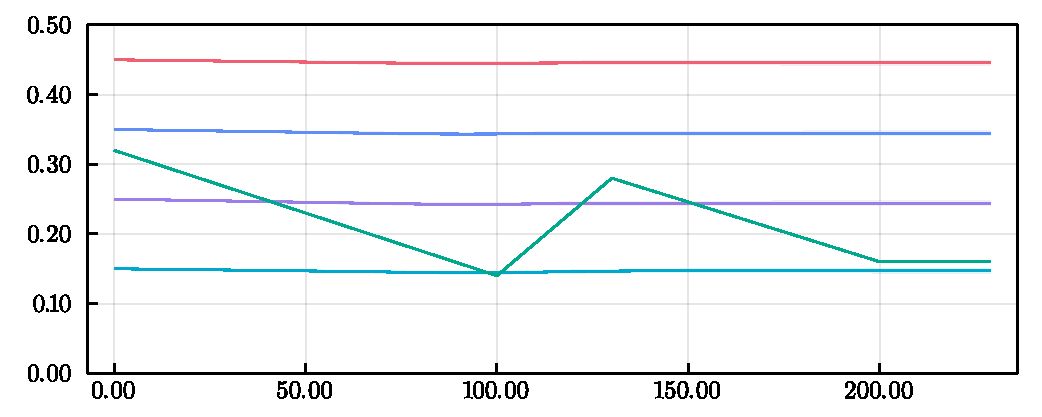
\includegraphics[width=\textwidth]{img/resultados/synth/sensialphacov_alphacov0-003_0alphaini0-15_0-1_0-45_high1_b2real1-88_gereal0-1961_gireal0-1389_acov0-8_aini0-27675_gcov0-05gamma_e_0-1961_gamma_i_0-1389_beta_2_1-8800.pdf}
     \caption{Estimación control clase 1, usando varianza para \(\alpha\) \(20^{-2.0}\)}
     \label{fig:legend-sensi-acov-class1--a}
\end{subfigure} 
\hfill
\begin{subfigure}[b]{0.47\textwidth}
     \centering
     %\includegraphics[width=\textwidth]{img/resultados/synth/sensialphacov_alphacov0-008\stringsensiacov\stringparamfour.pdf}
     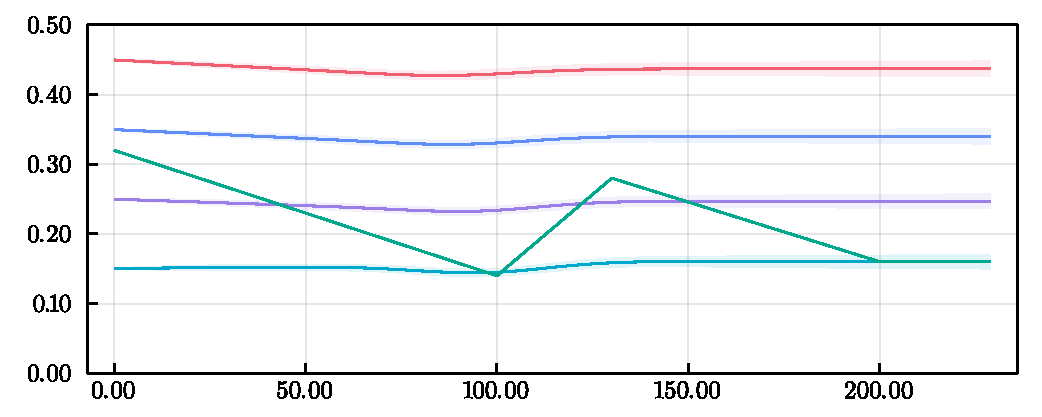
\includegraphics[width=\textwidth]{img/resultados/synth/sensialphacov_alphacov0-008_0alphaini0-15_0-1_0-45_high1_b2real1-88_gereal0-1961_gireal0-1389_acov0-8_aini0-27675_gcov0-05gamma_e_0-1961_gamma_i_0-1389_beta_2_1-8800.pdf}
     \caption{Estimación control clase 1, usando varianza para \(\alpha\) \(20^{-1.6}\)}
     \label{fig:legend-sensi-acov-class1--b}
\end{subfigure} 
\hfill
\begin{subfigure}[b]{0.47\textwidth}
     \centering
     %\includegraphics[width=\textwidth]{img/resultados/synth/sensialphacov_alphacov0-027\stringsensiacov\stringparamfour.pdf}
     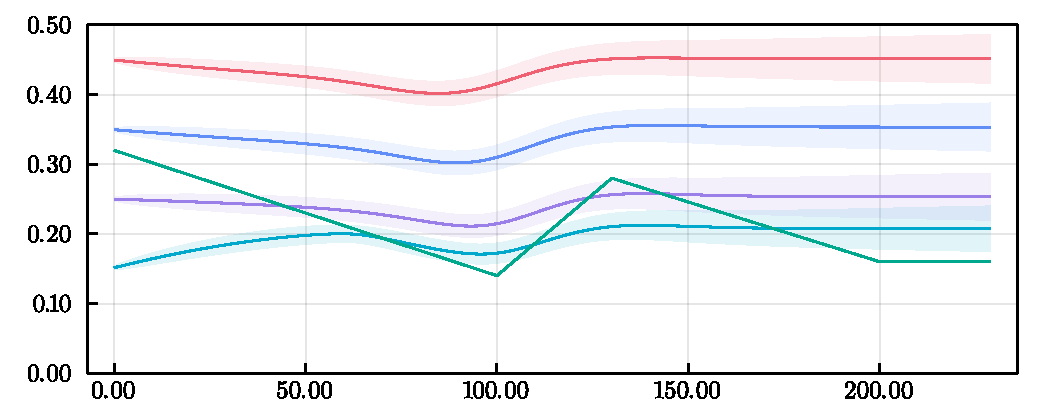
\includegraphics[width=\textwidth]{img/resultados/synth/sensialphacov_alphacov0-027_0alphaini0-15_0-1_0-45_high1_b2real1-88_gereal0-1961_gireal0-1389_acov0-8_aini0-27675_gcov0-05gamma_e_0-1961_gamma_i_0-1389_beta_2_1-8800.pdf}
     \caption{Estimación control clase 1, usando varianza para \(\alpha\) \(20^{-1.2}\)}
     \label{fig:legend-sensi-acov-class1--c}
\end{subfigure} 
\hfill
\begin{subfigure}[b]{0.47\textwidth}
     \centering
     %\includegraphics[width=\textwidth]{img/resultados/synth/sensialphacov_alphacov0-091\stringsensiacov\stringparamfour.pdf}
     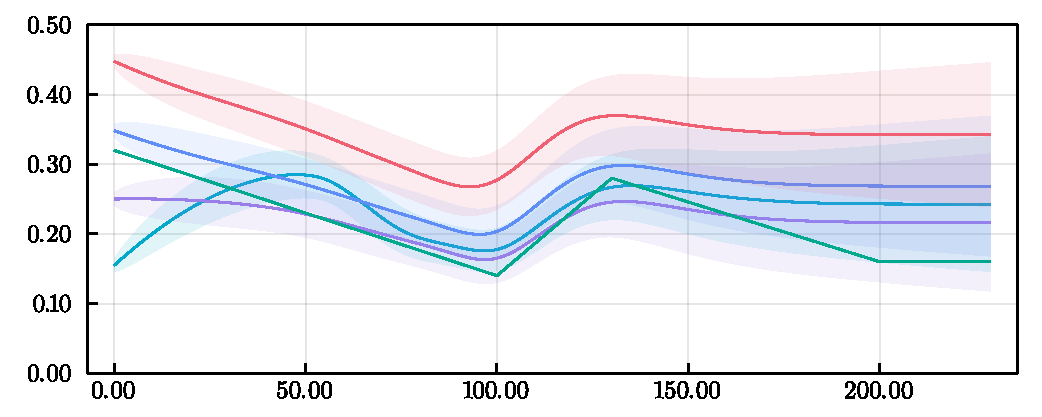
\includegraphics[width=\textwidth]{img/resultados/synth/sensialphacov_alphacov0-091_0alphaini0-15_0-1_0-45_high1_b2real1-88_gereal0-1961_gireal0-1389_acov0-8_aini0-27675_gcov0-05gamma_e_0-1961_gamma_i_0-1389_beta_2_1-8800.pdf}
     \caption{Estimación control clase 1, usando varianza para \(\alpha\) \(20^{-0.8}\)}
     \label{fig:legend-sensi-acov-class1--d}
\end{subfigure} 
\hfill
\begin{subfigure}[b]{0.47\textwidth}
     \centering
     %\includegraphics[width=\textwidth]{img/resultados/synth/sensialphacov_alphacov0-302\stringsensiacov\stringparamfour.pdf}
     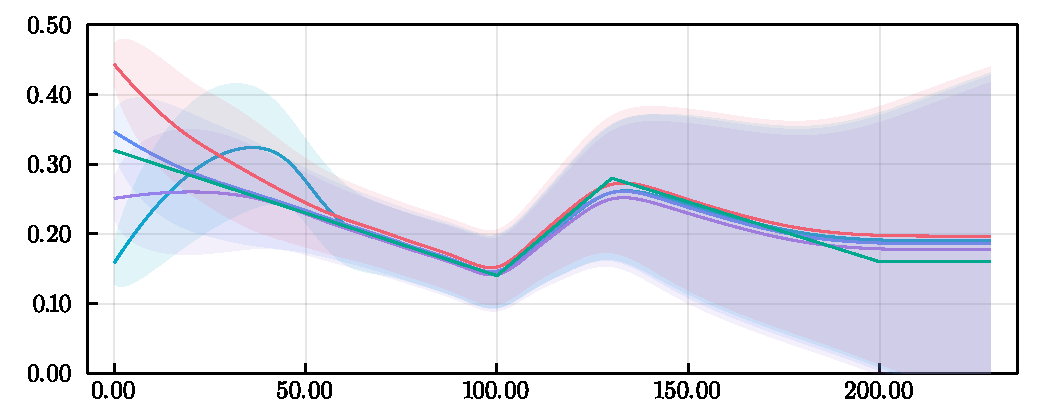
\includegraphics[width=\textwidth]{img/resultados/synth/sensialphacov_alphacov0-302_0alphaini0-15_0-1_0-45_high1_b2real1-88_gereal0-1961_gireal0-1389_acov0-8_aini0-27675_gcov0-05gamma_e_0-1961_gamma_i_0-1389_beta_2_1-8800.pdf}
     \caption{Estimación control clase 1, usando varianza para \(\alpha\) \(20^{-0.4}\)}
     \label{fig:legend-sensi-acov-class1--e}
\end{subfigure} 
\hfill
\begin{subfigure}[b]{0.47\textwidth}
     \centering
     %\includegraphics[width=\textwidth]{img/resultados/synth/sensialphacov_alphacov1-000\stringsensiacov\stringparamfour.pdf}
     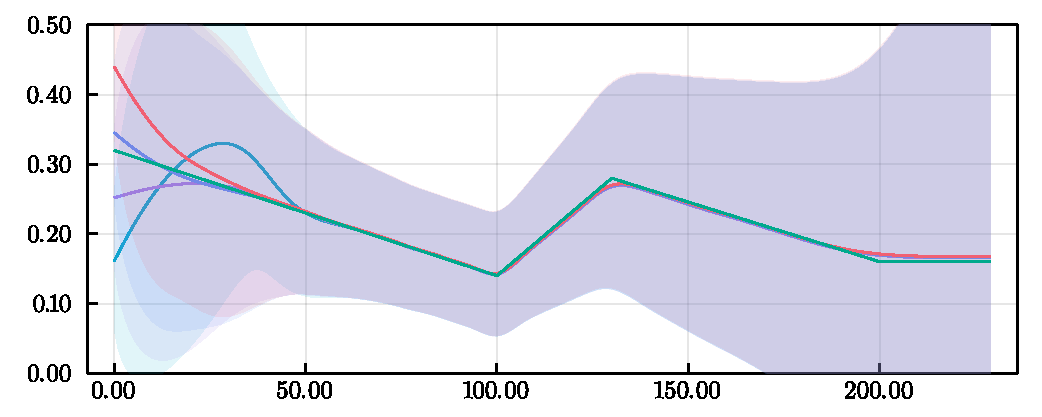
\includegraphics[width=\textwidth]{img/resultados/synth/sensialphacov_alphacov1-000_0alphaini0-15_0-1_0-45_high1_b2real1-88_gereal0-1961_gireal0-1389_acov0-8_aini0-27675_gcov0-05gamma_e_0-1961_gamma_i_0-1389_beta_2_1-8800.pdf}
     \caption{Estimación control clase 1, usando varianza para \(\alpha\) \(20^{0.0}\)}
     \label{fig:legend-sensi-acov-class1--f}
\end{subfigure} 
\hfill
\begin{subfigure}[b]{0.75\textwidth}
 \centering
\scalebox{0.7}{
\begin{tikzpicture}
	\begin{pgfonlayer}{nodelayer}
		\node [style=none] (0) at (-0.5, 1.25) {};
		\node [style=none] (1) at (1, 1.25) {};
		\node [style=none] (2) at (-0.5, 0.75) {};
		\node [style=none] (3) at (1, 0.75) {};
		\node [style=none] (4) at (-0.5, 0.25) {};
		\node [style=none] (5) at (1, 0.25) {};
		\node [style=none] (6) at (-0.5, -0.25) {};
		\node [style=none] (7) at (1, -0.25) {};
		\node [style=none] (8) at (1.5, 1.25) {$0.15$};
		\node [style=none] (9) at (1.5, 0.75) {};
		\node [style=none] (10) at (1.5, 0.75) {};
		\node [style=none] (11) at (1.5, 0.75) {$0.25$};
		\node [style=none] (12) at (1.5, 0.25) {};
		\node [style=none] (13) at (1.5, 0.25) {$0.35$};
		\node [style=none] (15) at (1.5, -0.25) {$0.45$};
		\node [style=none] (17) at (0.5, 1.75) {Condición inicial $\alpha_0$};
		\node [style=none] (21) at (6.5, 1) {};
		\node [style=none] (22) at (5.5, 0.5) {};
		\node [style=none] (23) at (7, 0.5) {};
		\node [style=none] (24) at (7.5, 0.5) {};
		\node [style=none] (25) at (7.5, 0.5) {Solución real};
	\end{pgfonlayer}
	\begin{pgfonlayer}{edgelayer}
		\draw [style={a0_1}] (0.center) to (1.center);
		\draw [style={a0_2}] (2.center) to (3.center);
		\draw [style={a0_3}] (4.center) to (5.center);
		\draw [style={a0_4}] (6.center) to (7.center);
		\draw [style=real] (22.center) to (23.center);
	\end{pgfonlayer}
\end{tikzpicture}
}
\end{subfigure}
\caption[Sensibilidad ante la varianza y condición inicial del factor sanitario.]{Sensibilidad ante la varianza y condición inicial del factor sanitario. Cada color representa una condición inicial diferente usada en la estimación.} \label{fig:legend-sensi-alphacov}
\end{figure}

Se recuerda que se hizo la simplificación de que los ruidos en la dinámica son independientes, es decir que el ruido está dado por una matriz normal multivariada con matriz de covarianzas diagonal. Nos interesa por tanto, solo la diagonal de la matriz, las varianzas. Se muestra el efecto en la estimación al usar distintos valores para la matriz de varianzas.

La figura \ref{fig:legend-sensi-alphacov} muestra la estimación del factor sanitario para distintos valores de varianza del ruido en la dinámica de este. Este valor refleja la certeza que tenemos en la dinámica del estado; si hay mucha, se usa una varianza baja. Si no hay tanta seguridad, se usa una varianza mayor, de tal forma de incorporar la información de los datos. Los gráficos  \ref{fig:legend-sensi-acov-class1--a} y \ref{fig:legend-sensi-acov-class1--b}  muestran lo que ocurre al utilizar una varianza demasiado baja en el estado aumentado; la estimación es muy insensible a los datos, y se queda muy cercana a la condición inicial dada. Tanto en \ref{fig:legend-sensi-acov-class1--c} como en \ref{fig:legend-sensi-acov-class1--d} ya va siendo posible percibir variaciones en el control, pero aún no se ve convergencia desde las distintas condiciones iniciales. Finalmente, los gráficos  \ref{fig:legend-sensi-acov-class1--e} y \ref{fig:legend-sensi-acov-class1--f} tienen suficiente varianza, como se ve en la convergencia de las estimaciones a partir de \(t >=50\) aproximadamente, sin embargo \ref{fig:legend-sensi-acov-class1--f} usa una varianza excesiva, ya que pueden obtenerse resultados similares con una mayor certeza.



%\subsection{Efecto del \textit{smoother}}\label{subsec:smoother}

\subsection{Modelo con datos reales}\label{subsec:datosreales}

El estudio realizado en las subsecciones anteriores entrega herramientas para trabajar con el caso real.



\begin{table}[h!]
\centering
\begin{tabular}{|| m{1cm} m{3cm} m{8cm}||} 
 \hline
 & \textbf{Fecha} & \textbf{Evento} \\
 \hline 
 (1) & 13/may/2020 & Comienzo de la cuarentena total en la RM.\\
 (2) & 28/jul/2020 & Comienza a regir el Plan Paso a Paso.\\
 (3) & 04/ene/2021 & Comienza a funcionar el pase de vacaciones.\\ 
 (4) & 03/feb/2021 & Comienza campaña de vacunación masiva (ver \ref{}).\\
 (5) & 26/may/2021 &  Un 50\% de la población en la RM tiene la primera dosis de la vacuna. \\
 \hline
\end{tabular}
\caption{Algunas fechas relevantes para el desarrollo de la pandemia en Santiago.}
\label{table:fechas-relevantes}
\end{table}


\begin{figure}[H]
\centering
\includegraphics[width=0.99\textwidth]{img/resultados/kalman_grouped_allstates_allgroups\parameterstring}
\caption[\textit{Kalman RTS Smoother} aplicado al caso real ]{\textit{Kalman RTS Smoother} aplicado al caso real. Se utiliza el Producto 15 de casos acumulados confirmados}
\label{all-nohigh}
\end{figure}



\begin{figure}[H]
     \centering
     \begin{subfigure}[b]{0.47\textwidth}
         \centering
         \includegraphics[width=\textwidth]{img/resultados/kalman_grouped_I_high1\parameterstring}
         \caption{Clase \(1\).}
     \end{subfigure}
     \hfill
     \begin{subfigure}[b]{.47\textwidth}
         \centering
         \includegraphics[width=\textwidth]{img/resultados/kalman_grouped_I_high2\parameterstring}
         \caption{Clase \(2\).}
     \end{subfigure}
     \hfill
     \begin{subfigure}[b]{.47\textwidth}
         \centering
         \includegraphics[width=\textwidth]{img/resultados/kalman_grouped_I_high3\parameterstring}
         \caption{Clase \(3\).}
     \end{subfigure}
     \hfill
     \begin{subfigure}[b]{.47\textwidth}
         \centering
         \includegraphics[width=\textwidth]{img/resultados/kalman_grouped_I_high4\parameterstring}
         \caption{Clase \(4\).}
     \end{subfigure}
     \hfill
     \begin{subfigure}[b]{.47\textwidth}
         \centering
         \includegraphics[width=\textwidth]{img/resultados/kalman_grouped_I_high5\parameterstring}
         \caption{Clase \(5\).}
     \end{subfigure}
     \hfill
     \begin{subfigure}[b]{.47\textwidth}
         \centering
         \includegraphics[width=\textwidth]{img/resultados/kalman_grouped_I_allclass\parameterstring}
         \caption{Todas las clases.}
     \end{subfigure}
        \caption{Cantidad de Infectados estimados a partir de datos reales, en valores absolutos y normalizados con respecto a la cantidad de personas por clase.}
        \label{e-comp-high}
\end{figure}



\begin{figure}[H]
     \centering
     \begin{subfigure}[b]{0.47\textwidth}
         \centering
         \includegraphics[width=\textwidth]{img/resultados/kalman_grouped_S_high1\parameterstring}
         \caption{Clase \(1\).}
     \end{subfigure}
     \hfill
     \begin{subfigure}[b]{.47\textwidth}
         \centering
         \includegraphics[width=\textwidth]{img/resultados/kalman_grouped_S_high2\parameterstring}
         \caption{Clase \(2\).}
     \end{subfigure}
     \hfill
     \begin{subfigure}[b]{.47\textwidth}
         \centering
         \includegraphics[width=\textwidth]{img/resultados/kalman_grouped_S_high3\parameterstring}
         \caption{Clase \(3\).}
     \end{subfigure}
     \hfill
     \begin{subfigure}[b]{.47\textwidth}
         \centering
         \includegraphics[width=\textwidth]{img/resultados/kalman_grouped_S_high4\parameterstring}
         \caption{Clase \(4\).}
     \end{subfigure}
     \hfill
     \begin{subfigure}[b]{.47\textwidth}
         \centering
         \includegraphics[width=\textwidth]{img/resultados/kalman_grouped_S_high5\parameterstring}
         \caption{Clase \(5\).}
     \end{subfigure}
     \hfill
     \begin{subfigure}[b]{.47\textwidth}
         \centering
         \includegraphics[width=\textwidth]{img/resultados/kalman_grouped_S_allclass\parameterstring}
         \caption{Todas las clases.}
     \end{subfigure}
        \caption{Cantidad de Susceptibles estimados a partir de datos reales, en valores absolutos y normalizados con respecto a la cantidad de personas por clase.}
        \label{s-comp-high}
\end{figure}




\begin{figure}[H]
     \centering
     \begin{subfigure}[b]{.99\textwidth}
         \centering
         \includegraphics[width=\textwidth]{img/resultados/kalman_grouped_alpha_allclass\parameterstring}
         \caption{Todas las clases.}
     \end{subfigure}
     \hfill
     \begin{subfigure}[b]{0.47\textwidth}
         \centering
         \includegraphics[width=\textwidth]{img/resultados/kalman_grouped_alpha_high1\parameterstring}
         \caption{Clase \(1\).}
     \end{subfigure}
     \hfill
     \begin{subfigure}[b]{.47\textwidth}
         \centering
         \includegraphics[width=\textwidth]{img/resultados/kalman_grouped_alpha_high2\parameterstring}
         \caption{Clase \(2\).}
     \end{subfigure}
     \hfill
     \begin{subfigure}[b]{.47\textwidth}
         \centering
         \includegraphics[width=\textwidth]{img/resultados/kalman_grouped_alpha_high3\parameterstring}
         \caption{Clase \(3\).}
     \end{subfigure}
     \hfill
     \begin{subfigure}[b]{.47\textwidth}
         \centering
         \includegraphics[width=\textwidth]{img/resultados/kalman_grouped_alpha_high4\parameterstring}
         \caption{Clase \(4\).}
     \end{subfigure}
     \hfill
     \begin{subfigure}[b]{.47\textwidth}
         \centering
         \includegraphics[width=\textwidth]{img/resultados/kalman_grouped_alpha_high5\parameterstring}
         \caption{Clase \(5\).}
     \end{subfigure}
        \caption[Factor sanitario estimado a partir de datos reales.]{Factor sanitario estimado a partir de datos reales. Las líneas grises corresponden a las fechas relevantes de la tabla \ref{table:fechas-relevantes}.}
        \label{alpha-comp-high}
\end{figure}


El estudio de sensibilidad mostró que los resultados dependen en mayor medida de \(\gamma_I\), y que \(\gamma_E\) solo produce variaciones muy pequeñas en el factor sanitario. Con esto en mente, la figura \ref{sensi-gammai-real} muestra la sensibilidad de los resultados con respecto a la variable \(\gamma_I\). Si bien la relación entre los factores sanitario no se mantiene constante en cada caso, sí se observa claramente que la Clase sin prioridad, o la más acomodada, disminuye considerablemente su riesgo mucho antes que las demás.

\begin{figure}[H]
     \centering
     \begin{subfigure}[b]{.47\textwidth}
         \centering
         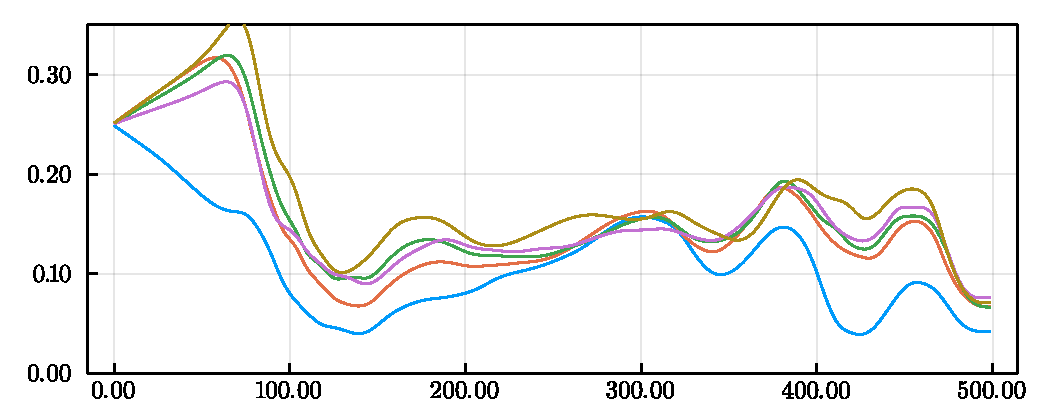
\includegraphics[width=\textwidth]{img/resultados/sensigammai_6-5_0alphaini0-15_0-1_0-45_high1__acov0-8_aini0-27675_gcov0-05gamma_e_0-1724_gamma_i_0-1389_beta_2_2-0000.pdf}
         \caption{\(1/\gamma_I = 6.5 [\text{días}]\)}
     \end{subfigure}
     \hfill
     \begin{subfigure}[b]{0.47\textwidth}
         \centering
         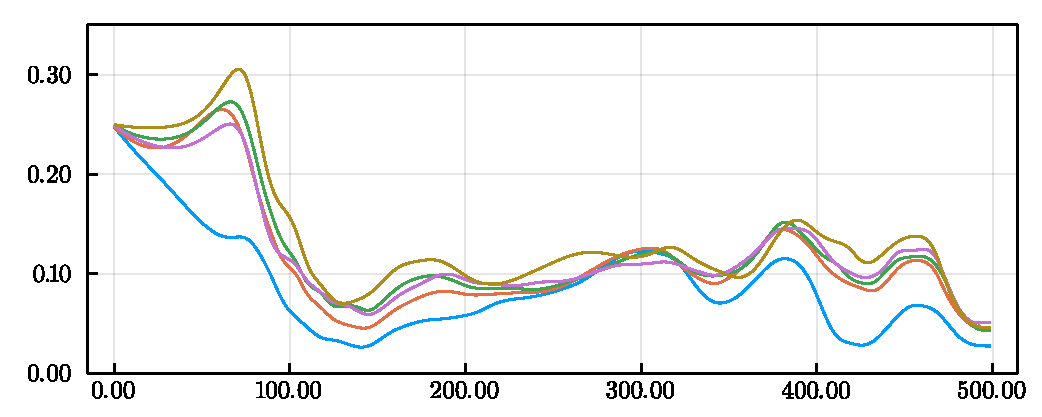
\includegraphics[width=\textwidth]{img/resultados/sensigammai_8-5_0alphaini0-15_0-1_0-45_high1__acov0-8_aini0-27675_gcov0-05gamma_e_0-1724_gamma_i_0-1389_beta_2_2-0000.pdf}
         \caption{\(1/\gamma_I = 8.5 [\text{días}]\)}
     \end{subfigure}
     \hfill
     \begin{subfigure}[b]{.47\textwidth}
         \centering
         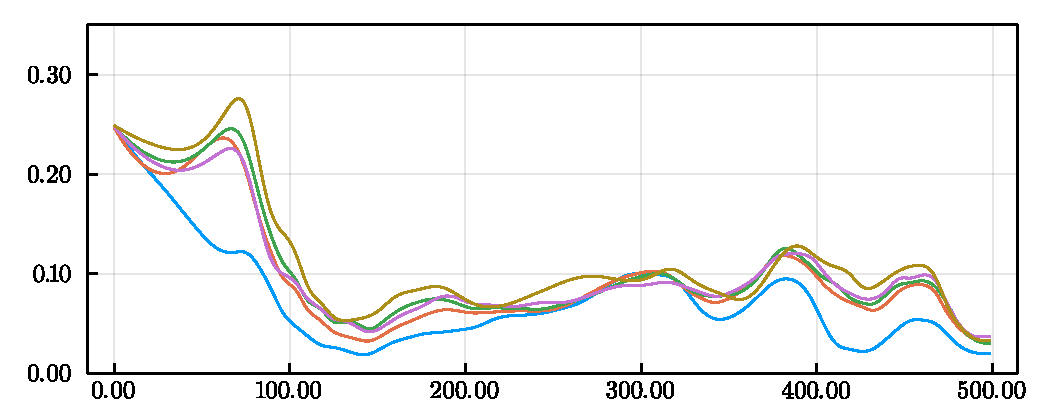
\includegraphics[width=\textwidth]{img/resultados/sensigammai_10-5_0alphaini0-15_0-1_0-45_high1__acov0-8_aini0-27675_gcov0-05gamma_e_0-1724_gamma_i_0-1389_beta_2_2-0000.pdf}
         \caption{\(1/\gamma_I = 10.5 [\text{días}]\)}
     \end{subfigure}
     \hfill
     \begin{subfigure}[b]{.47\textwidth}
         \centering
         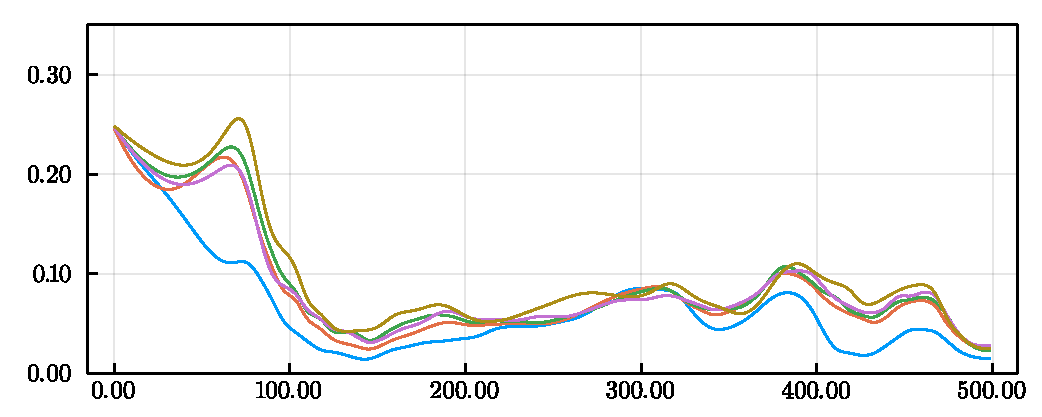
\includegraphics[width=\textwidth]{img/resultados/sensigammai_12-5_0alphaini0-15_0-1_0-45_high1__acov0-8_aini0-27675_gcov0-05gamma_e_0-1724_gamma_i_0-1389_beta_2_2-0000.pdf}
         \caption{\(1/\gamma_I = 12.5 [\text{días}]\)}
     \end{subfigure}
     \hfill
     \begin{subfigure}[b]{.47\textwidth}
         \centering
         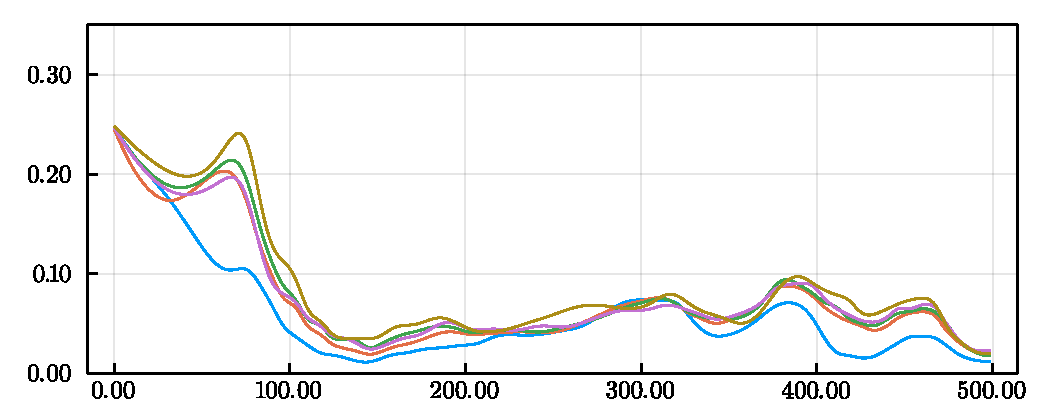
\includegraphics[width=\textwidth]{img/resultados/sensigammai_14-5_0alphaini0-15_0-1_0-45_high1__acov0-8_aini0-27675_gcov0-05gamma_e_0-1724_gamma_i_0-1389_beta_2_2-0000.pdf}
         \caption{\(1/\gamma_I = 14.5 [\text{días}]\)}
     \end{subfigure}
     \hfill
    \caption[Sensibilidad factor sanitario estimado para los datos reales, ante distintos \(\gamma_I\).]{}
    \label{sensi-gammai-real}
\end{figure}




% Agrupar para usar datos reales, calcular Rt y comparar con Cori
\section{Evaluación del modelo mediante casos hipotéticos}\label{sec:evalmodel-casoshipot}

% Descripción de los tipos de cuarentena y las medidas de cuidado 
Las combinaciones entre los distintos niveles de cuidado y cuarentena presentados en \ref{met:evaluacion} dan lugar a una serie de casos, los cuales son presentados en la tabla \ref{table:casos-hipoteticos}. Se resuelve el sistema de ecuaciones diferenciales ordinarias \ref{eq:modelo-final} para cada caso, utilizando las distintas variantes de \(\alpha_i(t)\) y \(P(t)\), modificadas a partir de las estimaciones logradas en la sección anterior.

\begin{table}[h!]
\centering
\begin{tabular}{||l| c c c||} 
 \hline
 & \textbf{Cuidado insuficiente} & \begin{tabular}{@{}c@{}}\textbf{Cuidado} \\ \textbf{normal}\end{tabular} & \begin{tabular}{@{}c@{}}\textbf{Cuidado} \\ \textbf{extra}\end{tabular}\\ 
 \hline
 \textbf{Sin cuarentena} & Caso 1 & Caso 2 & Caso 3 \\ 
 \textbf{Cuarentena normal} & Caso 4 & Caso 5 & Caso 6 \\
 \textbf{Cuarentena fuerte} & Caso 7 & Caso 8 & Caso 9 \\
 \hline
\end{tabular}
\caption{Casos hipotéticos para distintas combinaciones de cuarentena y cuidado.}
\label{table:casos-hipoteticos}
\end{table}


Se prueban dos escenarios. En el primero de ellos, \(\beta_{\text{exterior}}\) es un valor mucho más grande que \(1\), de forma que la tasa de contagio está totalmente dominada por el ambiente exterior y prácticamente todos los contagios ocurren fuera de casa. Este se estudia en la subsección \ref{eval:beta-grande}. En el segundo, \(\beta_{\text{exterior}}\) es un valor mayor pero cercano a \(1\), de tal forma que el ambiente hogar contribuye a la tasa de contagios. Este se estudia en \ref{eval:beta-chico}.


\subsection{Escenario con contagio exterior predominante}\label{eval:beta-grande}


En este escenario se considera \(\beta_{\text{exterior}} >> 1\), de forma que la tasa de contagio está totalmente dominada por el ambiente exterior y las infecciones ocurren solamente en el exterior del hogar, las infecciones dentro del hogar son despreciables en comparación. Se utiliza \(\beta_{\text{exterior}} = 68.0\), pero los resultados son similares para un rango amplio de parámetros.

% Las figuras \ref{img:all-hip-S-N} y \ref{img:all-hip-I-N} presentan la evolución de los susceptibles \(S_i/N_i\) e infectados \(S_i/N_i\) (normalizados por el total de personas en cada clase), para cada uno de los casos. Se utilizan los mismos límites para los ejes \(y\) para facilitar la comparación.

Como era de esperarse, las diferencias socioeconómicas en la incidencia disminuyen debido a que la mayoría de los casos están utilizando, o bien la misma matriz de tiempos de residencia, o bien los mismos factores sanitarios, o incluso ambos.

La tabla \ref{table:descripcion-casos-hipot} describe los resultados para los distintos casos considerados, tomando como referencia el caso 5, de cuarentena y cuidado normal. En los casos 1 y 2, que corresponden a casos sin cuarentena con cuidado insuficiente o cuidado normal respectivamente, se contagia la gran mayoría de la población dentro de los primeros 6 meses considerados. En el caso con cuidado normal, la clase más acomodada resulta tener una incidencia bastante menor que las demás.

El cuidado extra logra contener la enfermedad con cuarentena normal o fuerte, como muestran los casos 6 y 9. La enfermedad desaparece rápidamente de entre la población en los primeros meses, aunque esto desde luego no considera importación de casos externos.

\begin{table}[H]
\centering
\begin{tabular}{||m{2.5cm}|m{4cm} m{4cm} m{4cm}||} 
 \hline
 & \begin{tabular}{@{}c@{}}\textbf{Cuidado} \\ \textbf{insuficiente}\end{tabular} & \begin{tabular}{@{}c@{}}\textbf{Cuidado} \\ \textbf{normal}\end{tabular} & \begin{tabular}{@{}c@{}}\textbf{Cuidado} \\ \textbf{extra}\end{tabular}\\ 
 \hline
 \textbf{Sin cuarentena} & \textit{Caso 1}: Se contagia un \(90\%\) de la población en los primeros 6 meses, de manera uniforme entre las distintas clases. Luego la enfermedad desaparece. & \textit{Caso 2}: Se contagia un \(65\%\) de la población de la clase alta en los primeros 6 meses, y un \(80\%\) de las demás clases. Luego la enfermedad desaparece. & \textit{Caso 3}: Se logra controlar el alza de casos, alcanzando el \textit{peak} de mediados de julio de 2020 y el de inicios de mayo de 2021 con menos de la mitad de casos, e incluso se evita el rebrote de junio de 2021. Ver figura \ref{img:esc-beta-grande-c3}.\\ 
 \textbf{Cuarentena normal} & \textit{Caso 4}: El primer \textit{peak} de julio de 2020 alcanza más del doble de casos y tiene una reducción lenta, de tal forma que el \textit{peak} de mayo de 2021 es apenas registrado como un alza ligera. Ver figura \ref{img:esc-beta-grande-c4}. & \textit{Caso 5}: Desarrollo real de la pandemia, tomado como referencia& \textit{Caso 6}: La enfermedad alcanza un pequeño \textit{peak} en julio de 2020 y luego se extingue.\\
 \textbf{Cuarentena fuerte} & \textit{Caso 7}: El primer \textit{peak} es muy similar en fecha y número de infectados, pero con un alza sostenida en el número de casos a partir septiembre de 2020, llegando a un \textit{peak} de más del doble de infectados en julio de 2021.  Ver figura \ref{img:esc-beta-grande-c7}. & \textit{Caso 8}: Se observan dos \textit{peaks} de unas 5000 personas, similar al Caso 3 pero sin poder contener el rebrote de junio de 2021. Ver figura \ref{img:esc-beta-grande-c8}. & \textit{Caso 9}: La enfermedad se extingue luego de los primeros meses. \\
 \hline
\end{tabular}
\caption{Observaciones para cada caso hipotético, escenario con \(\beta_{\text{exterior}} = 68\).}
\label{table:descripcion-casos-hipot}
\end{table}




% Aquí pongo todos los resultados de casos hipotéticos que obtuve... cuarentenas fuertes, etc... 
% \begin{figure}[h]
% \centering
% \includegraphics[width=0.99\textwidth]{img/resultados/allhipcases_S-N_commonylim0_1\parameterstring}
% \caption{Estimación de susceptibles, normalizados por el total de cada grupo \(S_i/N_i\), para cada caso hipotético.}
% \label{img:all-hip-S-N}
% \end{figure}

% \begin{figure}[h]
% \centering
% \includegraphics[width=0.99\textwidth]{img/resultados/allhipcases_I-N_commonylim0-015\parameterstring}
% \caption{Estimación de infectados normalizados por el total de cada grupo \(I_i/N_i\), para cada caso hipotético.}
% \label{img:all-hip-I-N}
% \end{figure}

La figura \ref{img:hip-3478-I-comp} muestra cuatro casos interesantes, comparándolos con la situación normal. En estos tres casos, el impacto es mayor sobre la clase 5 (prioridad alta, la más vulnerable). Esto puede atribuirse al hecho de que esa es la clase que presenta en general un mayor factor sanitario y movilidad, por lo que se verían más favorecidos si pudieran guardar las cuarentenas o las medidas de cuidado de mejor manera.
 
 El caso 3, que puede verse en \ref{img:esc-beta-grande-c3}, es interesante, ya que propone que la pandemia pudo controlarse incluso sin cuarentena, siempre y cuando todos pudieran evitar las aglomeraciones, usar mascarilla, lavado de manos y mantenerse lejos de los demás. El caso 4, en la figura \ref{img:esc-beta-grande-c4}, plantea que las medidas de higiene y cuidado sí fueron importantes, y que evitaron un \textit{peak} de más del doble de casos en los primeros meses de la pandemia. 
 
 
El caso 7, en la figura \ref{img:esc-beta-grande-c7}, afirma que una cuarentena más fuerte habría compensado una falta de preocupación o capacidad de cumplimiento de las medidas de higiene y cuidado, al menos en los primeros meses. La situación se desborda a medida que se acerca el 2021, debido a que la población sale del confinamiento. El caso 8, en la figura \ref{img:esc-beta-grande-c8}, es muy similar al caso 3, pero no logra evitar un segundo \textit{peak} en julio de 2021.

% Fechas 
% important_dates = [
%    Date(2020, 5, 13), # cuarentena total en la RM
%    Date(2020, 10, 25), # plesbicito por nueva constitución
%    Date(2021, 1, 4), # comienza a regir el permiso de vacaciones
%    Date(2021, 2, 1), # comienza un plan de vacunación más fuerte (según datos)
%    Date(2021, 5, 26) # un 50% de la población de Santiago tiene la primera dosis
%]
% casos interesantes: 3, 4, 7, 8

\begin{figure}[H]
     \centering
     \begin{subfigure}[b]{.47\textwidth}
         \centering
         \includegraphics[width=\textwidth]{img/resultados/comparecase_3withnormal_I_\parameterstring}
         \caption{Caso \(3\): Cuidado extra sin cuarentena.}
         \label{img:esc-beta-grande-c3}
     \end{subfigure}
     \hfill
     \begin{subfigure}[b]{.47\textwidth}
         \centering
         \includegraphics[width=\textwidth]{img/resultados/comparecase_4withnormal_I_\parameterstring}
         \caption{Caso \(4\): Cuidado insuficiente y cuarentena normal.}
         \label{img:esc-beta-grande-c4}
     \end{subfigure}
     \hfill
     \begin{subfigure}[b]{.47\textwidth}
         \centering
         \includegraphics[width=\textwidth]{img/resultados/comparecase_7withnormal_I_\parameterstring}
         \caption{Caso \(7\): Cuidado insuficiente y cuarentena fuerte.}
         \label{img:esc-beta-grande-c7}
     \end{subfigure}
     \hfill
     \begin{subfigure}[b]{.47\textwidth}
         \centering
         \includegraphics[width=\textwidth]{img/resultados/comparecase_8withnormal_I_\parameterstring}
         \caption{Caso \(8\): Cuidado normal y cuarentena fuerte.}
         \label{img:esc-beta-grande-c8}
     \end{subfigure}
     \hfill 
    \begin{subfigure}[b]{0.99\textwidth}
    \centering
    \scalebox{0.7}{
    \begin{tikzpicture}
	\begin{pgfonlayer}{nodelayer}
		\node [style=none] (50) at (5, 0) {};
		\node [style=none] (51) at (7, 0) {};
		\node [style=none] (52) at (6, -0.5) {Prioridad Alta};
		\node [style=none] (53) at (2, 0) {};
		\node [style=none] (54) at (4, 0) {};
		\node [style=none] (55) at (3, -0.5) {Prioridad};
		\node [style=none] (56) at (-1, 0) {};
		\node [style=none] (57) at (1, 0) {};
		\node [style=none] (58) at (0, -0.5) {Prioridad};
		\node [style=none] (59) at (-4, 0) {};
		\node [style=none] (60) at (-2, 0) {};
		\node [style=none] (61) at (-3, -0.5) {Prioridad Baja};
		\node [style=none] (62) at (-7, 0) {};
		\node [style=none] (63) at (-5, 0) {};
		\node [style=none] (64) at (-6, -0.5) {Sin Prioridad};
		\node [style=none] (65) at (0, -1) {Media Baja};
		\node [style=none] (66) at (3, -1) {Media Alta};
	\end{pgfonlayer}
	\begin{pgfonlayer}{edgelayer}
		\draw [style=class5] (50.center) to (51.center);
		\draw [style=class1] (62.center) to (63.center);
		\draw [style=class2] (59.center) to (60.center);
		\draw [style=class3] (56.center) to (57.center);
		\draw [style=class4] (53.center) to (54.center);
	\end{pgfonlayer}
\end{tikzpicture}

    }
    \end{subfigure}
        \caption[Personas infectadas para casos hipotéticos seleccionados. Escenario \(\beta_{\text{exterior}} >> 1\).]{Personas infectadas para caso hipotéticos seleccionados, con la estimación de los casos reales de fondo. Diferentes límites para el eje \(y\). Las líneas grises corresponden a las fechas relevantes de la tabla \ref{table:fechas-relevantes}.}
        \label{img:hip-3478-I-comp}
\end{figure}


\subsection{Escenario con contagio en hogar}\label{eval:beta-chico}


En este caso se buscó un valor donde existiera contagio en el hogar, y se eligió \(\beta_{\text{exterior}} = 1.2\). Esto se hizo estudiando las contribuciones de los ambientes a la tasa de contagio, calculando las contribuciones a la derivada de cada ambiente dadas por \ref{eq:contribuciones-j}, en la subsección \ref{met-subsec:fijos}. Bajo estas condiciones, se observa que la cuarentena prácticamente no influye en el número de contagios; lo que realmente determina si se controla o no la pandemia es el factor sanitario. Los resultados se sintetizan en la tabla \ref{table:descripcion-casos-hipot-beta-1-2}, y los casos de interés elegidos anteriormente se presentan en la figura \ref{img:hip-3478-I-comp-beta1-2}.



\begin{table}[h!]
\centering
\begin{tabular}{||m{2.5cm}|m{4cm} m{4cm} m{4cm}||} 
 \hline
 & \begin{tabular}{@{}c@{}}\textbf{Cuidado} \\ \textbf{insuficiente}\end{tabular}  & \begin{tabular}{@{}c@{}}\textbf{Cuidado} \\ \textbf{normal}\end{tabular} & \begin{tabular}{@{}c@{}}\textbf{Cuidado} \\ \textbf{extra}\end{tabular}\\ 
 \hline
 \textbf{Con o sin cuarentena} & \textit{Casos 1, 4 y 7}: Se observan \textit{peaks} de más del doble de casos que el normal, y que se reducen más lentamente. El número de contagios no baja del \(0.5\%\) de la población. Ver figuras \ref{img:esc-beta-chico-c4} y \ref{img:esc-beta-chico-c7}. & \textit{Caso 2, 5 y 8} Muy similares al caso 5, el normal usado como referencia. Ver figura \ref{img:esc-beta-chico-c8}. & \textit{Caso 3, 6, y 9}: La enfermedad tiene un pequeño \textit{peak} en torno a julio de 2020 y se extingue luego de unos meses. Ver figura \ref{img:esc-beta-chico-c3}. \\
 \hline
\end{tabular}
\caption[Observaciones para cada caso hipotético, escenario con \(\beta_{\text{exterior}} = 1.2\)]{Observaciones para cada caso hipotético, escenario con \(\beta_{\text{exterior}} = 1.2\). Tabla condensada, puesto que no hay variaciones importantes con respecto a la fuerza de la cuarentena.}
\label{table:descripcion-casos-hipot-beta-1-2}
\end{table}



\begin{figure}
     \centering
     \begin{subfigure}[b]{.47\textwidth}
         \centering
         \includegraphics[width=\textwidth]{img/resultados/comparecase_3withnormal_I_gamma_e_0-1724_gamma_i_0-0833_beta_2_2-0000.pdf}
         \caption{Caso \(3\): Cuidado extra sin cuarentena.}
         \label{img:esc-beta-chico-c3}
     \end{subfigure}
     \hfill
     \begin{subfigure}[b]{.47\textwidth}
         \centering
         \includegraphics[width=\textwidth]{img/resultados/comparecase_4withnormal_I_gamma_e_0-1724_gamma_i_0-0833_beta_2_2-0000.pdf}
         \caption{Caso \(4\): Cuidado insuficiente y cuarentena normal.}
         \label{img:esc-beta-chico-c4}
     \end{subfigure}
     \hfill
     \begin{subfigure}[b]{.47\textwidth}
         \centering
         \includegraphics[width=\textwidth]{img/resultados/comparecase_7withnormal_I_gamma_e_0-1724_gamma_i_0-0833_beta_2_2-0000.pdf}
         \caption{Caso \(7\): Cuidado insuficiente y cuarentena fuerte.}
         \label{img:esc-beta-chico-c7}
     \end{subfigure}
     \hfill
     \begin{subfigure}[b]{.47\textwidth}
         \centering
         \includegraphics[width=\textwidth]{img/resultados/comparecase_8withnormal_I_gamma_e_0-1724_gamma_i_0-0833_beta_2_2-0000.pdf}
         \caption{Caso \(8\): Cuidado normal y cuarentena fuerte.}
         \label{img:esc-beta-chico-c8}
     \end{subfigure}
     \hfill
    \begin{subfigure}[b]{0.99\textwidth}
    \centering
    \scalebox{0.6}{
    \begin{tikzpicture}
	\begin{pgfonlayer}{nodelayer}
		\node [style=none] (50) at (5, 0) {};
		\node [style=none] (51) at (7, 0) {};
		\node [style=none] (52) at (6, -0.5) {Prioridad Alta};
		\node [style=none] (53) at (2, 0) {};
		\node [style=none] (54) at (4, 0) {};
		\node [style=none] (55) at (3, -0.5) {Prioridad};
		\node [style=none] (56) at (-1, 0) {};
		\node [style=none] (57) at (1, 0) {};
		\node [style=none] (58) at (0, -0.5) {Prioridad};
		\node [style=none] (59) at (-4, 0) {};
		\node [style=none] (60) at (-2, 0) {};
		\node [style=none] (61) at (-3, -0.5) {Prioridad Baja};
		\node [style=none] (62) at (-7, 0) {};
		\node [style=none] (63) at (-5, 0) {};
		\node [style=none] (64) at (-6, -0.5) {Sin Prioridad};
		\node [style=none] (65) at (0, -1) {Media Baja};
		\node [style=none] (66) at (3, -1) {Media Alta};
	\end{pgfonlayer}
	\begin{pgfonlayer}{edgelayer}
		\draw [style=class5] (50.center) to (51.center);
		\draw [style=class1] (62.center) to (63.center);
		\draw [style=class2] (59.center) to (60.center);
		\draw [style=class3] (56.center) to (57.center);
		\draw [style=class4] (53.center) to (54.center);
	\end{pgfonlayer}
\end{tikzpicture}

    }
    \end{subfigure}
        \caption[Personas infectadas para caso hipotéticos seleccionados.]{Personas infectadas para caso hipotéticos seleccionados, con la estimación de los casos reales de fondo. Diferentes límites para el eje \(y\). Las líneas grises corresponden a las fechas relevantes de la tabla \ref{table:fechas-relevantes}.}
        \label{img:hip-3478-I-comp-beta1-2}
\end{figure}


% Esto ya es solo una pregunta... pero se puede hacer el proceso a la inversar? obtener estimaciones de movilidad para distintos grupos usando los datos de infecciones.... el problema es que el mejor indicador son los fallecidooooos y los resultados dependen mucho de las tasas de muerte.
